\documentclass[submit,techreq,noauthor]{eco}	% ゼミ用テンプレート
% \documentclass[submit,techreq,noauthor,dvipdfmx]{b3-eco}	% b3用テンプレート
% \documentclass[submit,techreq,noauthor,dvipdfmx]{mid-eco}	% b4中間発表テンプレート

\usepackage[dvipdfmx]{graphicx}
\usepackage{mediabb}				% for pdf include
\usepackage{listings, jlisting} 		% for source code
\usepackage{url}
\usepackage{setspace}
\usepackage{enumitem}
\usepackage{booktabs}

% フォントの警告を無視
\usepackage{silence}
\WarningFilter{latexfont}{Some font shapes}
\WarningFilter{latexfont}{Font shape}

% listingsの設定
\lstset{
	%プログラム言語(複数の言語に対応,C,C++も可)
 	% language = C++,
 	%枠外に行った時の自動改行
 	breaklines = true,
 	%自動改行後のインデント量(デフォルトでは20[pt])
 	breakindent = 10pt,
 	%標準の書体
 	basicstyle = \ttfamily\scriptsize,
 	%コメントの書体
 	commentstyle = {\itshape \color[cmyk]{1,0.4,1,0}},
 	%関数名等の色の設定
 	% classoffset = 0,
 	%キーワード(int, ifなど)の書体
 	% keywordstyle = {\bfseries \color[cmyk]{0,1,0,0}},
 	%表示する文字の書体
 	stringstyle = {\ttfamily \color[rgb]{0,0,1}},
 	%枠 "t"は上に線を記載, "T"は上に二重線を記載
	%他オプション:leftline,topline,bottomline,lines,single,shadowbox
 	frame = ltbr,
	%行番号の位置
	% numbers = left,
	%行番号の間隔
 	stepnumber = 1,
	%タブの大きさ
 	tabsize = 4,
}

% \setstretch{1.5} % 行間を広くします(資料チェックしてもらうときはコメントを外す)

\begin{document}

\semino {4/1}					% 年度/回数
\date   {4/4/1/火}				% 令和/月/日/曜日
\title  {地球環境に配慮した毛利研究室ゼミテンプレート}	% タイトル
\author {立命 太郎}				% 氏名


\begin{abstract}
	近年,地球の環境破壊が問題となっている.
	限りある資源を有効に活用するため,ペーパレスを推進する企業も増え始めている.
	我が毛利研究室でも,ゼミ資料の紙の使用量を抑制する動きが見られている.
	そこで,表紙を無くした新たなゼミテンプレートの作成を行った.
	本稿では,新しいゼミテンプレートと付録として添付したMakefileの使用法について述べる.
\end{abstract}
\maketitle

%%%%%%%%%%%%%%%%%%%%%ここから消して下さい%%%%%%%%%%%%%%%%%%%%%
\section{はじめに}
本稿では,
テンプレートのディレクトリ構成と
Makefileの概要や画像の挿入方法,参考文献の書き方について述べる.
資料をチェックしてもらうときは,本ファイル8行目の
\verb|\setstretch{1.5}|
のコメントを外すとチェックする側はありがたいです.
LaTexのコンパイル時にエラーが出るor文字化けする場合は,文字コードが原因の可能性が高いです.
テンプレートはUTF-8にしていますが,各自環境に合わせて設定して下さい.


\section{ディレクトリ構成}
ゼミテンプレートの構成は,以下に示す.
画像は,figフォルダへ入れる.
本文はsemi.texに記述,参考文献はreferences.bibにそれぞれ記述する.

\begin{lstlisting}
├─ Makefile		% Makefile
├─ eco.cls		% texのフォーマット
├─ fig/		% 画像保存用
│   ├── ex1.eps	% サンプル画像
│   └── ex2.pdf	% サンプル画像
├─ ipsjunsrt.bst	% 参考文献のスタイル
├─ jlisting.sty	% ソースコード添付用
├─ mediabb.sty 	% pdf変換用
├─ references.bib	% 参考文献
├─ semi.pdf		% 本文のPDF
└─ semi.tex		% 本文
\end{lstlisting}

\section{Makefileの概要}
make helpコマンドで使用方法が書いてあるので参考に.

PDFにを作成するには,make pdf とすると作成できる.
直接PDFを表示するには,make view とするとAdobe Readerで開いてくれる.

BibTeXでエラーが出た人は,Makefileの57行目の
\begin{lstlisting}
BIBTEX   := pbibtex
\end{lstlisting}
の部分をpbibtexからjbibtexに変更してみて下さい.
また,references.bibのファイルが存在しなければ,BibTeXは実行されません.
なので,BibTeXを使いたくない人は,references.bibを削除する(そんな人は卒論で苦労するよ).

文字コードを変更する場合は,make nkf-euc, make nkf-sjis, make nkf-utf8 コマンドでそれぞれ変更できます.

LaTeX,BibTeXでのlogを最後にまとめて表示するには,Makefileの45行目の
\begin{lstlisting}
JOIN-LOGS        := no
\end{lstlisting}
をyesにして下さい.このオプションを利用するにはrubyが必要です.


\section{参考文献の書き方}
参考文献は,BibTeXを使う.
たとえば,図\ref{fig:bibsample}の内容を含むファイル(references.bib)を作り,
\verb|\cite{etx}|の様に本文で参照\cite{etx}し,pbibtexコマンドで参考文献リストを作成します.
論文データベースには,必ずbibtex形式というのが用意されているはず.
その内容をコピーすれば基本は大丈夫なはず(必ずチェックする).
参考文献のスタイルは,情報処理学会の出現順のものを使用しています.

\begin{figure*}[t]
	\begin{lstlisting}
@INPROCEEDINGS{etx,
  author = {Douglas S. J. De Couto and Daniel Aguayo and John C. Bicket and Robert Morris},
  title = {A high-throughput path metric for multi-hop wireless routing},
  booktitle = {Proc. of ACM MobiCom '03},
  year = {2003},
  pages = {134-146}
}
    \end{lstlisting}
	\vspace{-2mm}
	\caption{BibTeXの記述例}
	\label{fig:bibsample}
\end{figure*}



\section{図の挿入方法}
\subsection{TgifやOpenOfficeで作る場合}
TgifやOpenOfficeで作る場合は,epsで出力して,includegraphicsで挿入しましょう(例:図\ref{fig:tgif-sample}).

\begin{figure}[t]
	\centering
	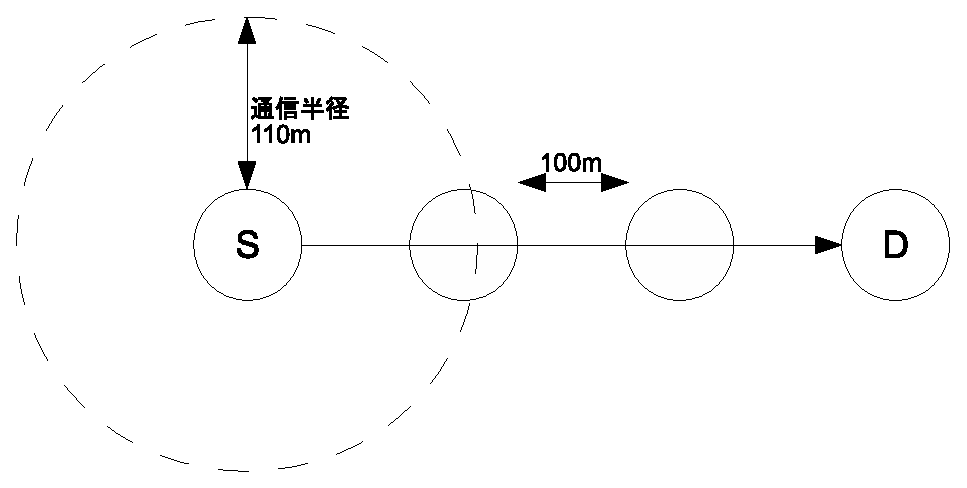
\includegraphics[width=8cm]{fig/ex1.eps}
	\caption{Open Officeで作成した図}
	\label{fig:tgif-sample}
\end{figure}

\subsection{PowerPointで作る場合}
複雑な図を作るときは,Microsoft PowerPointやVisioがおすすめ.
図をPDFでエクスポートし,それをTeXで表示できます(例: 図\ref{fig:pdf-sample}).
PDFを作成時にフォントが埋め込まれているかを確認する.
場合によっては,図のフォントが文字化けすることがあるので注意.

\begin{figure}[t]
	\centering
	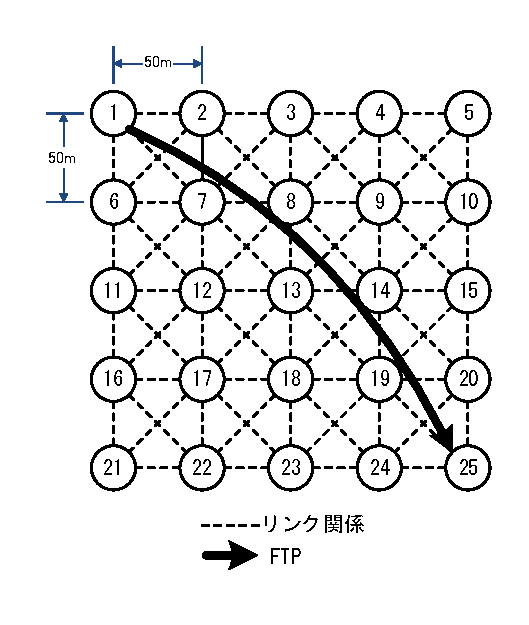
\includegraphics[width=8cm]{fig/ex2.pdf}
	\caption{PowerPointで作成した図}
	\label{fig:pdf-sample}
\end{figure}


\subsection{svgファイル}
svgを貼るときはincludegraphicsに拡張子を指定しない.
make実行時にpdfに変換されるため.
\begin{figure}[t]
	\centering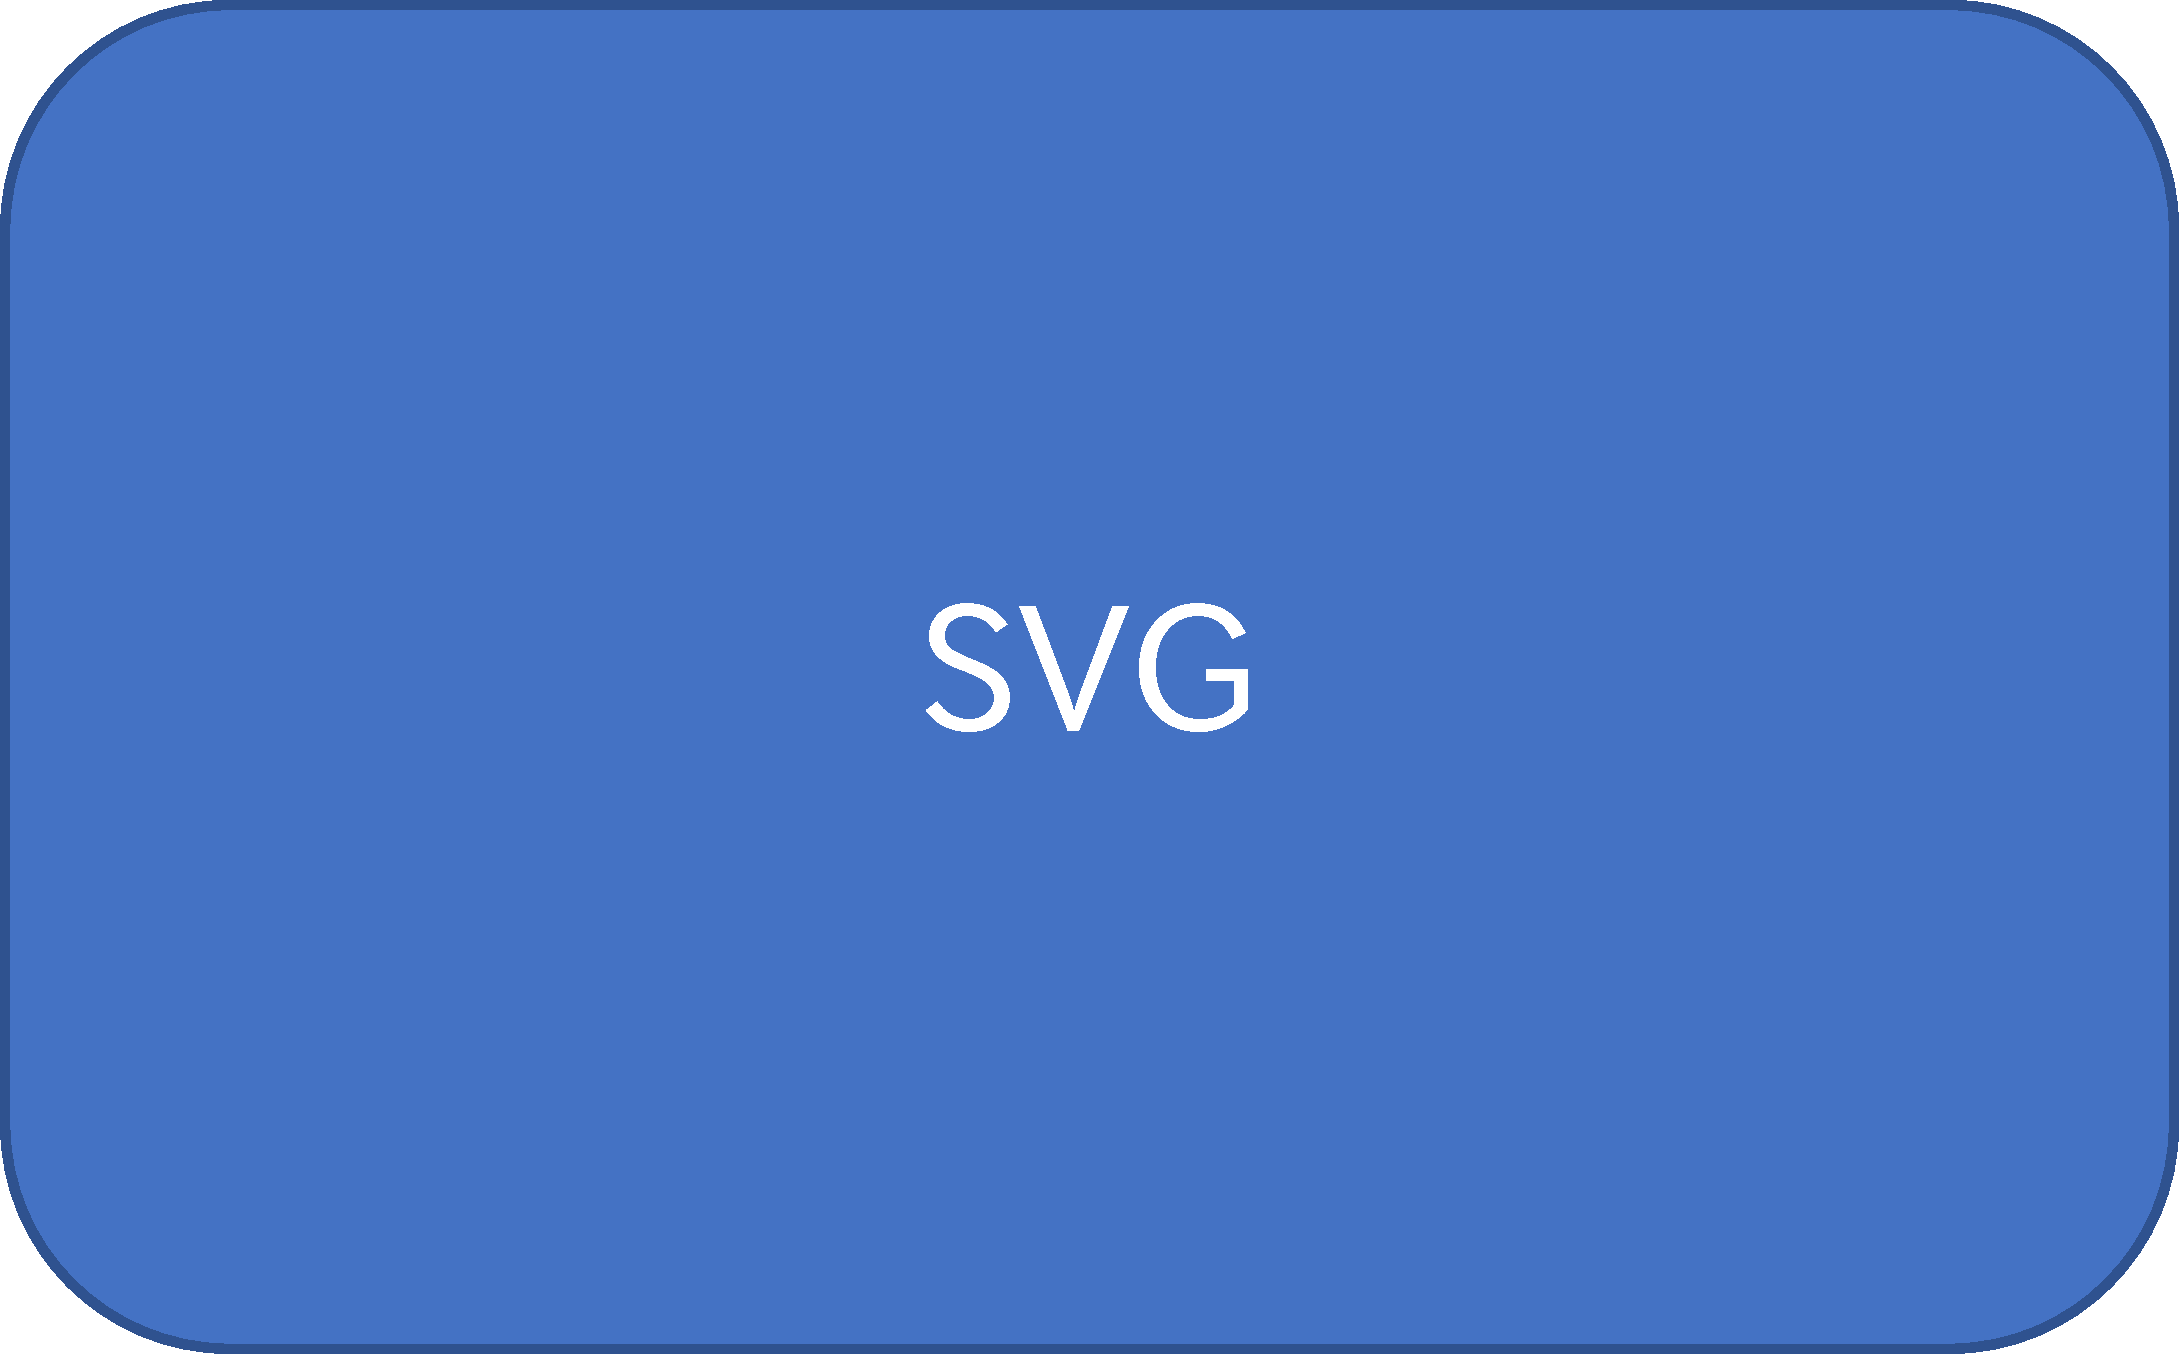
\includegraphics[width=80mm, angle=0]{fig/svg-sample}
	\caption{svgファイル}\label{fig:svg-sample}
\end{figure}



%%%%%%%%%%%%%%%%%%%%%ここまで消して下さい%%%%%%%%%%%%%%%%%%%%%

%bibtex
\setlength\baselineskip{12pt}
{\small
	\bibliography{references}
	\bibliographystyle{ipsjunsrt}
}


\end{document}